% !TEX root = ../../main.tex
%   \hspace{1.8cm}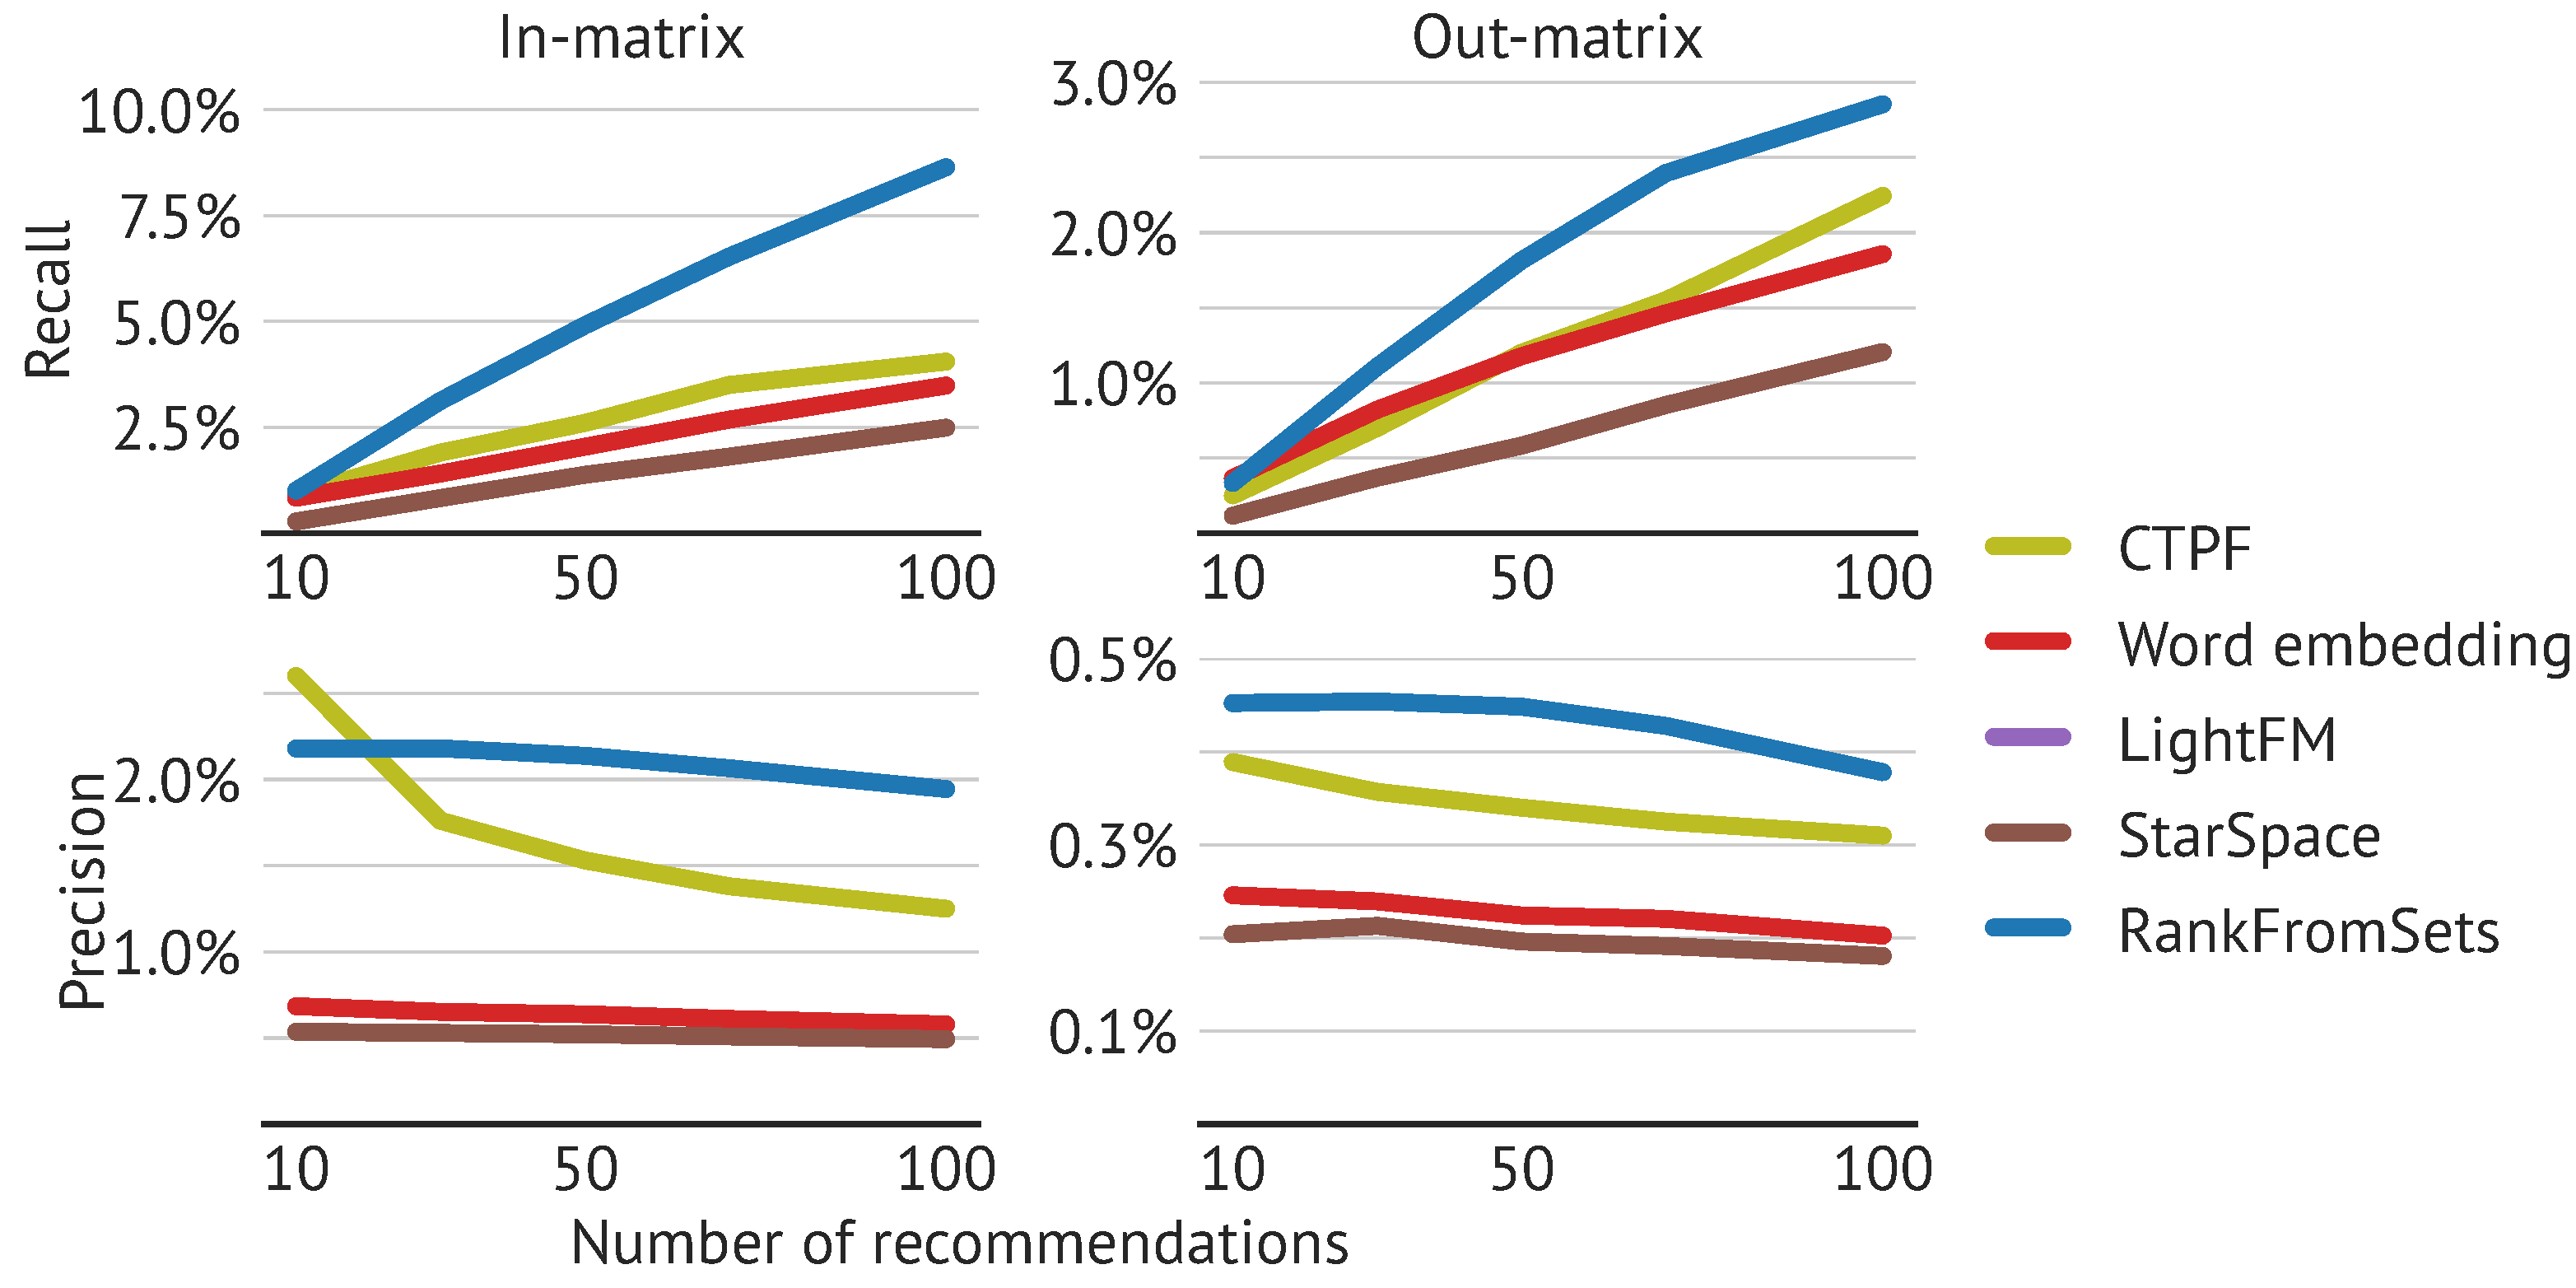
\includegraphics[width=0.7\linewidth]{ch-rfs/fig/arxiv}
\begin{figure*}[t]
  \centering
  \begin{subfigure}{\linewidth}
    \centering
    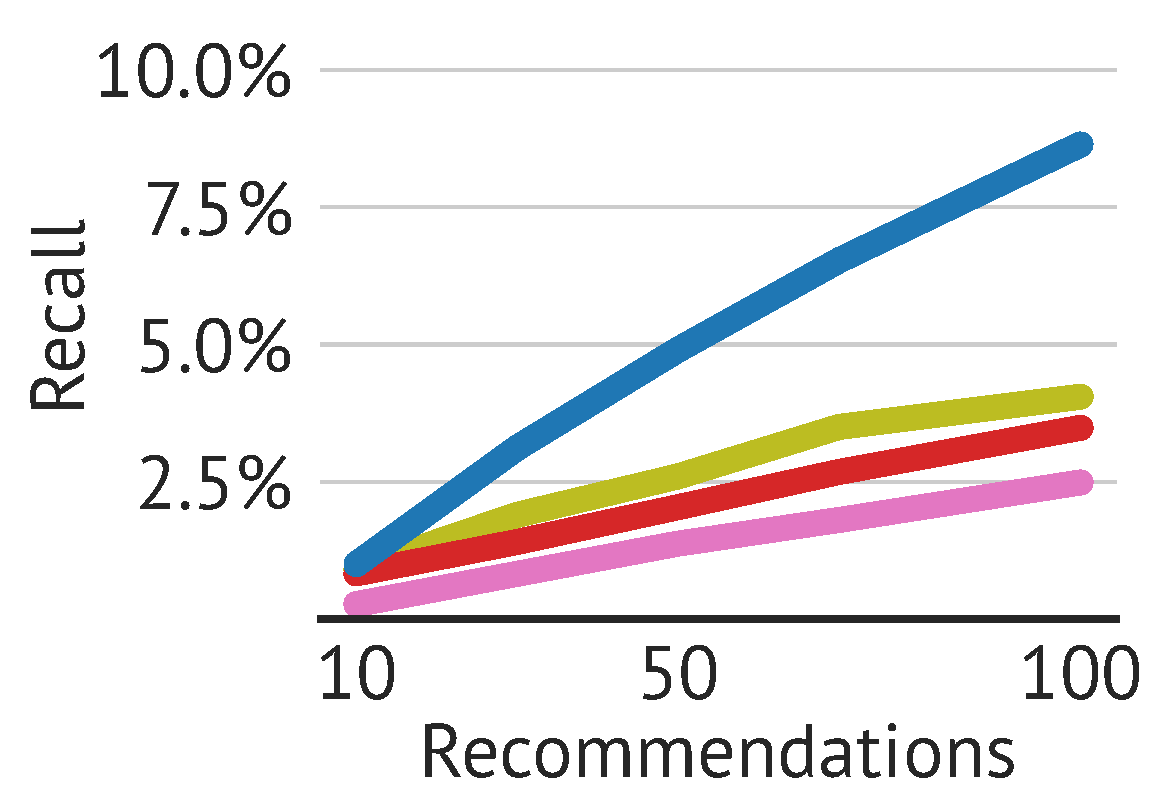
\includegraphics[width=.3\linewidth]{ch-rfs/fig/arxiv-in-matrix-recall}
    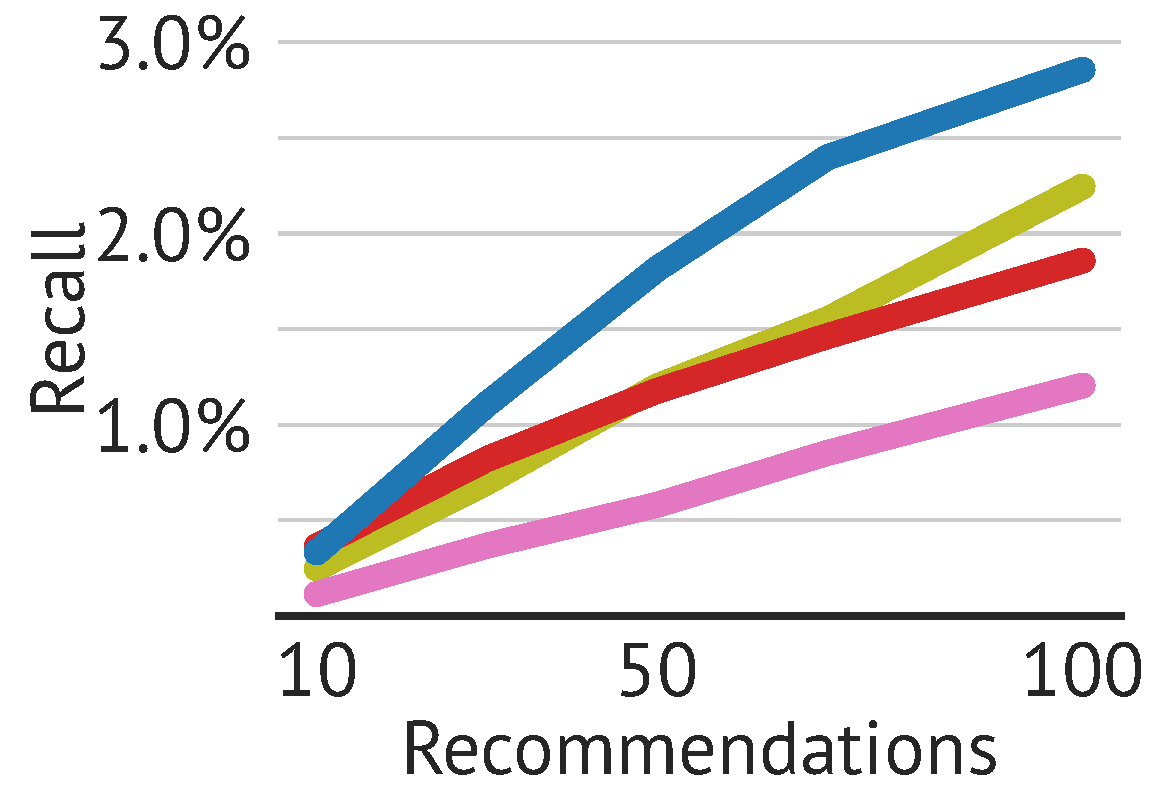
\includegraphics[width=.3\linewidth]{ch-rfs/fig/arxiv-out-matrix-recall}
    \hspace{3mm}
    \raisebox{9mm}{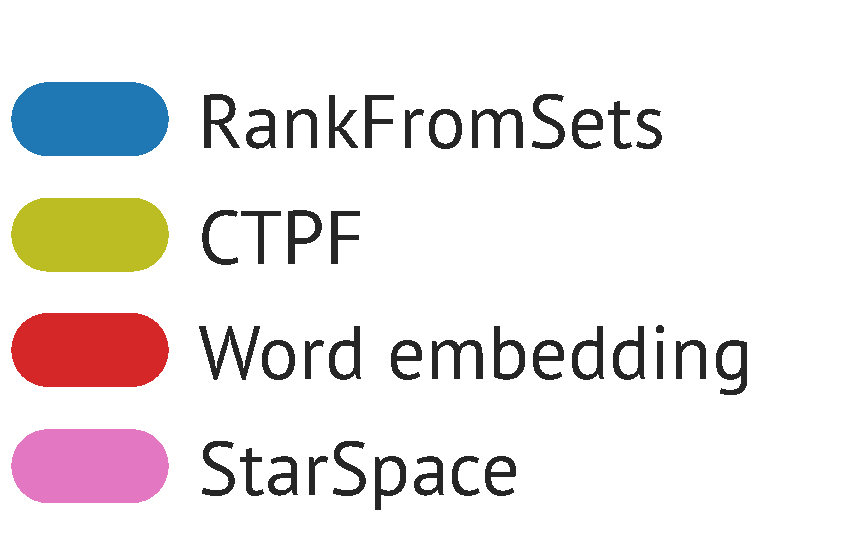
\includegraphics[width=0.2\linewidth]{ch-rfs/fig/arxiv-legend}}
    \caption{Recall for in-matrix (left) and out-matrix (right) documents.}
    \vspace*{0.5cm}
  \end{subfigure}
  \begin{subfigure}{\linewidth}
    \centering
    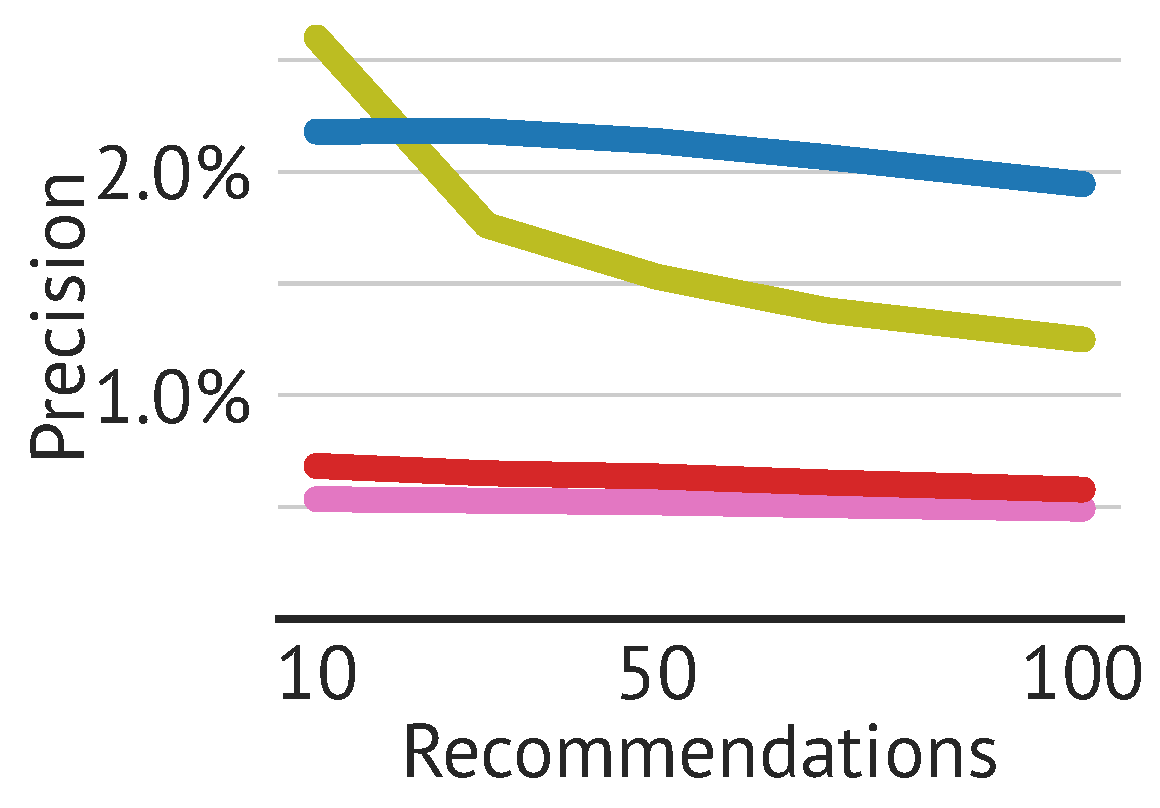
\includegraphics[width=.3\linewidth]{ch-rfs/fig/arxiv-in-matrix-precision}
    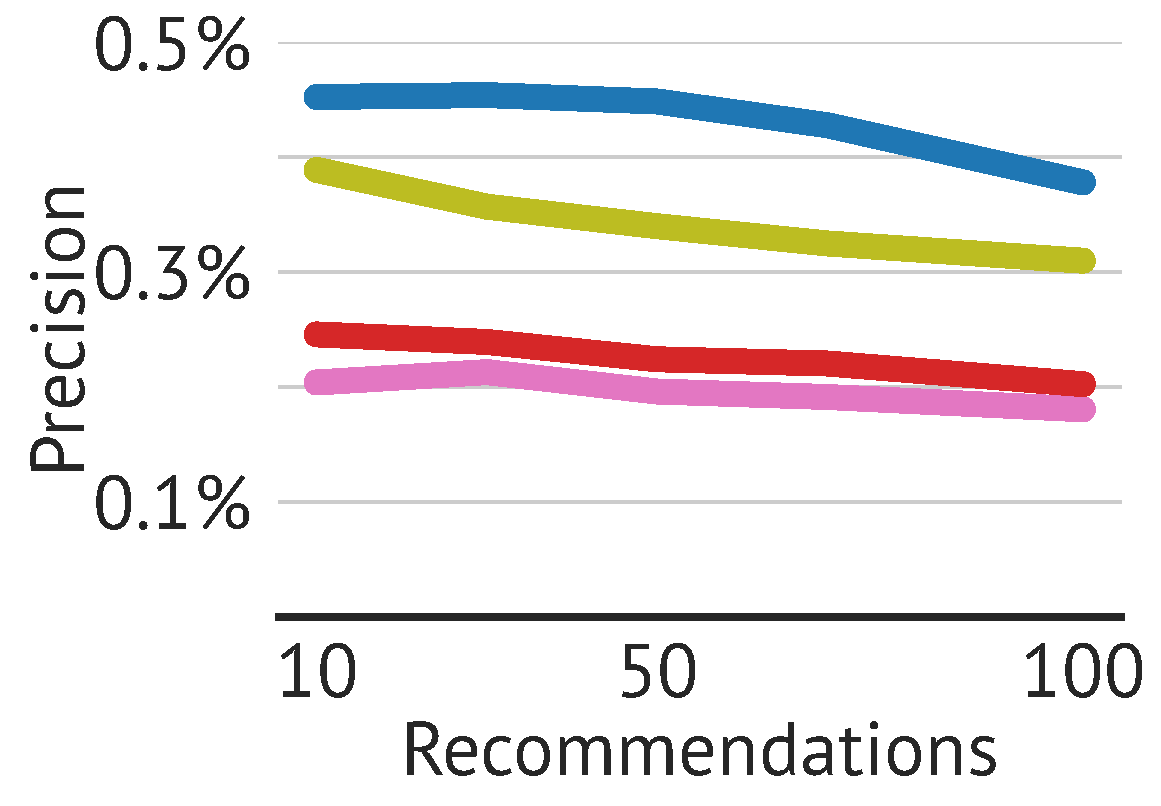
\includegraphics[width=.3\linewidth]{ch-rfs/fig/arxiv-out-matrix-precision}
    \hspace{3mm}
    \raisebox{9mm}{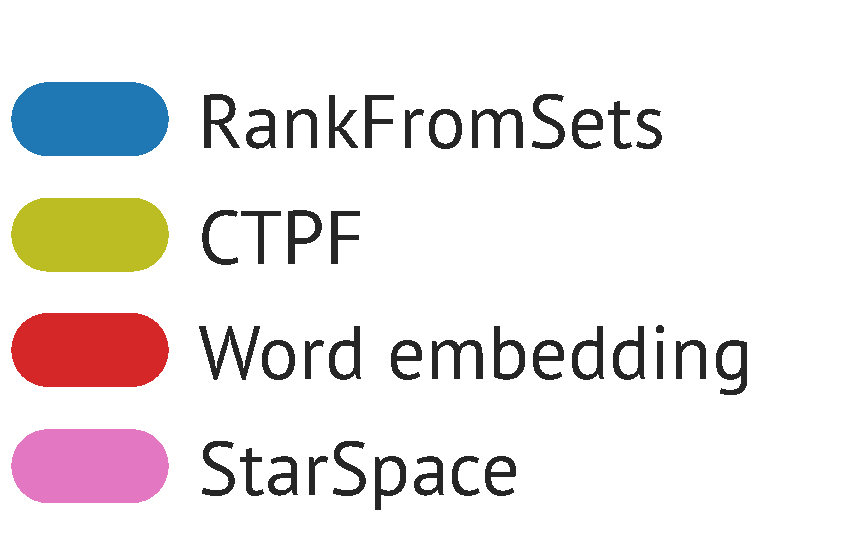
\includegraphics[width=0.2\linewidth]{ch-rfs/fig/arxiv-legend}}
    \caption{Precision for in-matrix (left) and out-matrix (right) documents.}
  \end{subfigure}
  % \begin{subfigure}[b]{\figwidthrfs}
  %   \centering
  %   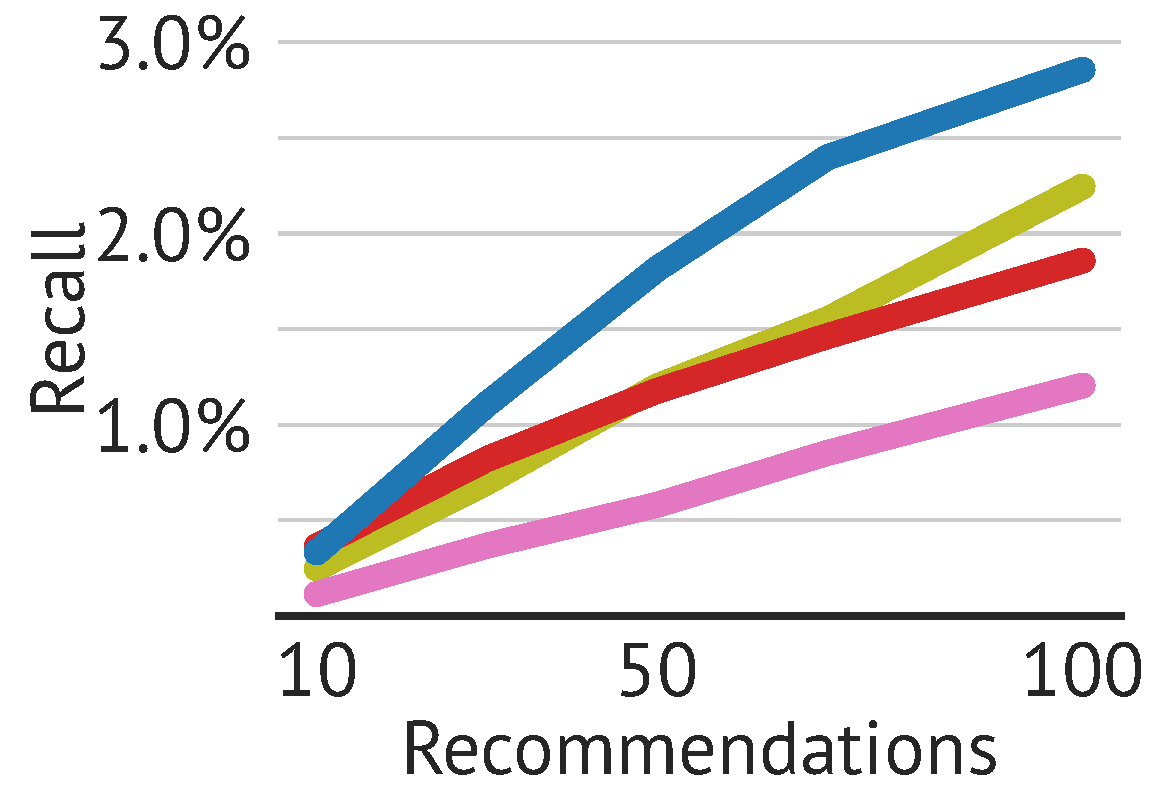
\includegraphics[width=\mysizerfs]{ch-rfs/fig/arxiv-out-matrix-recall}
  %   \caption{Out-matrix}%
  %   \label{fig:arxiv-out-recall}%
  % \end{subfigure}
  % \begin{subfigure}[b]{\figwidthrfs}
  %   \centering
  %   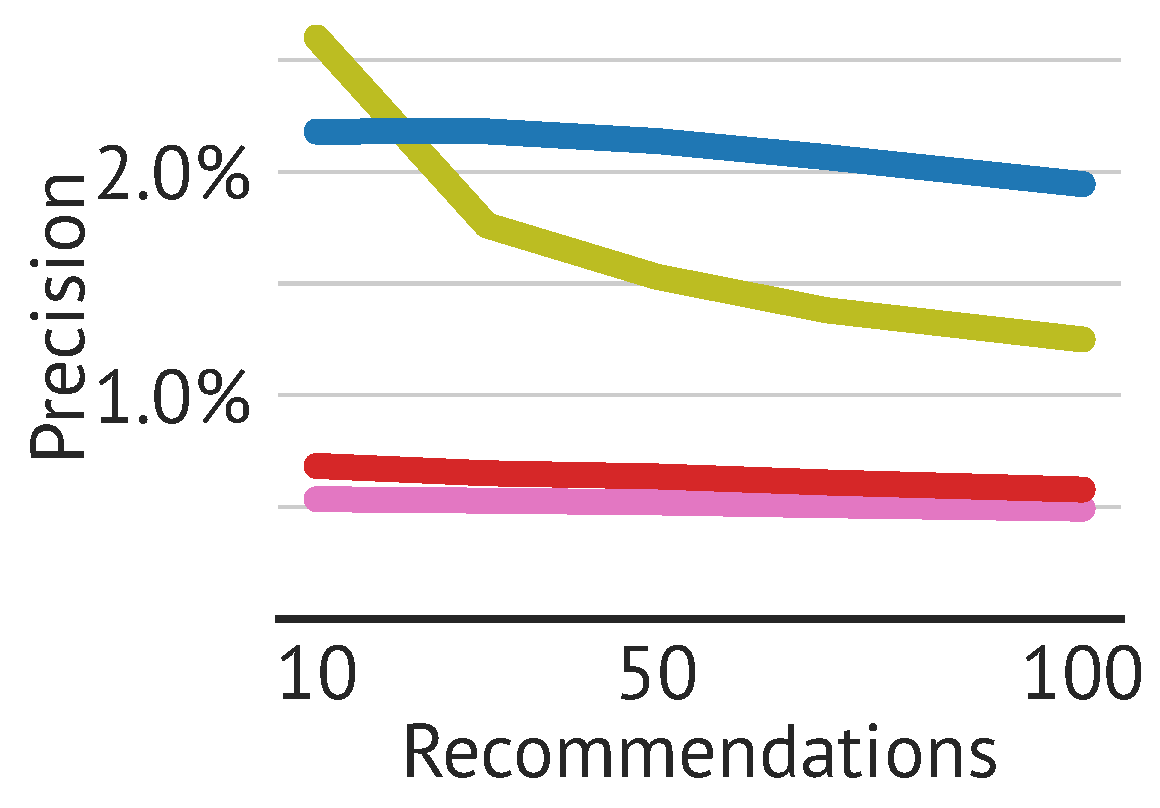
\includegraphics[width=\mysizerfs]{ch-rfs/fig/arxiv-in-matrix-precision}
  %   \caption{In-matrix}%
  %   \label{fig:arxiv-in-precision}%
  % \end{subfigure}
  % \begin{subfigure}[b]{\figwidthrfs}
  %   \centering
  %   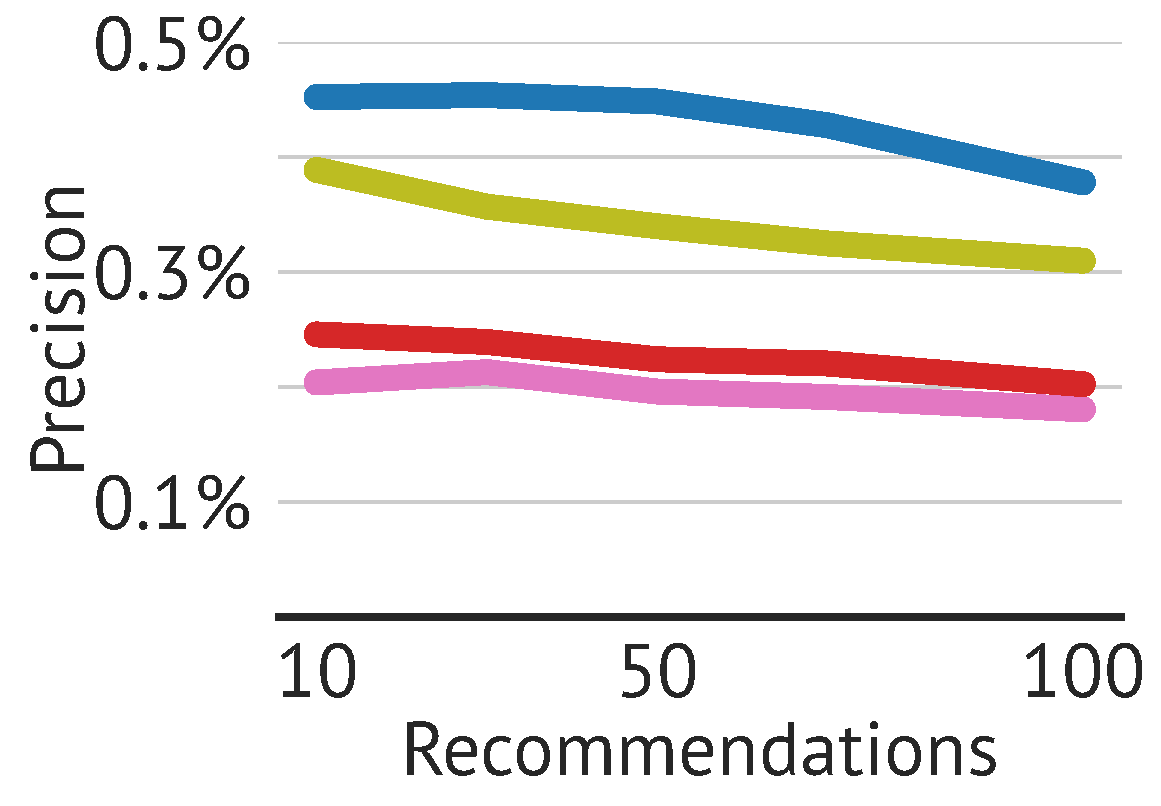
\includegraphics[width=\mysizerfs]{ch-rfs/fig/arxiv-out-matrix-precision}
  %   \caption{Out-matrix}%
  %   \label{fig:arxiv-out-precision}%
  % \end{subfigure}
  \caption[\textsc{rfs} results on arXiv data for article recommendation]{\label{fig:arxiv-performance} \textbf{\acrlong{rfs} outperforms collaborative topic Poisson factorization (\acrshort{ctpf})~\citep{gopalan2014content-based} and other models on recommending arXiv papers to scientists.} The items are documents and the attributes are the unique words in the abstracts. Recommendation performance is evaluated using both precision and recall to match the evaluation in \citep{gopalan2014content-based}. The metrics are reported on training (in-matrix) documents and cold-start (out-matrix) documents with no clicks in the training set. All \acrshort{gru} and \acrshort{lstm}-based models in \citet{bansal2016ask-the-gru:} performed an order of magnitude worse, and these results are omitted (training details are in \Cref{sec:appendix-empirical}).}
\end{figure*}